\chapter{Introduction}
\label{ch:intro}

\section{What \mcams\ does}

\mcams\ (Monte Carlo Attenuation and Multiple Scattering) is a Python package that simulates, with the Monte Carlo method, what happens to particles
(for example neutrons or X-ray photons) of a rectangular beam that crosses a
sample and is detected at a scattering angle $2\theta$. The sample is made of
layers, each one with its own material. Four geometries are available:
\begin{itemize}
  \item a \textbf{slab}: flat rectangular layers stacked one behind the other, which can be rotated
        around the vertical axis with respect to the beam;
  \item a \textbf{disc}: the same, but with a circular section centred on the beam, as a round flat cell or a pellet
        (version 2.3, Chapter~\ref{ch:disc});
  \item a \textbf{sphere}: concentric spheres (a full sphere surrounded by spherical shells) centred on the beam
        (version 2.4, Chapter~\ref{ch:sphere});
  \item a \textbf{cylinder}: concentric cylinders (a full inner cylinder surrounded by
        annular layers) with a vertical axis at the centre of the instrument.
\end{itemize}
In all the geometries every layer has its own \textbf{vertical extent}: its material lies between a bottom and a
top, measured from the centre of the beam, and the layer is empty below and above. This describes a container
that is not full, a powder resting on a support, or a container that starts inside the beam. Part of the beam
can then pass over or under the material (Chapter~\ref{ch:partial}).
The detector is the one of a two-axis instrument: it moves on a circle centred on
the sample, in the horizontal plane (Figure~\ref{fig:instrument}).

With the package you can answer questions such as:
\begin{enumerate}
  \item Where in the beam does each particle start? (Chapter~\ref{ch:beam})
  \item In which layer, and at which point, does a particle interact? (Chapters~\ref{ch:sample} and~\ref{ch:physics})
  \item What fraction of the scattered particles leaves the sample towards the detector,
        as a function of the angle? (Chapter~\ref{ch:transmission})
  \item How many particles reach the angle $2\theta$ after exactly one scattering, and how many
        after two or more? (Chapter~\ref{ch:scattering})
  \item How does that transmission depend on the layer in which the \emph{last} scattering
        happened? (Chapter~\ref{ch:lastlayer})
  \item Which are the attenuation coefficient and the scattering ratio of a layer, given its
        chemical formula, density and cross sections? (Chapter~\ref{ch:builder})
  \item How do all these results change when the container is only partially filled, or when the
        material does not start at the bottom of the beam? (Chapter~\ref{ch:partial})
  \item How does a round flat sample differ from a rectangular one? (Chapter~\ref{ch:disc})
  \item How does a spherical sample differ from a cylindrical one? (Chapter~\ref{ch:sphere})
  \item How do I compute the attenuation factors and the multiple scattering of a sample in a container inside a furnace, as
        \textsc{correct} does, but with the Monte Carlo? (Chapter~\ref{ch:correct})
  \item Which are the exact single-scattering attenuation factors of each layer, to use as a reference
        for the Monte Carlo? (Chapter~\ref{ch:direct})
\end{enumerate}

\begin{note}[New in version 2.0]
Layers of different heights, aligned on the bottom of the sample: each layer has a fill height, or a
\emph{fullness} (the fraction of the beam height covered by its material). The samples of earlier versions,
with all layers full, give the same numbers as before.
\end{note}

\begin{note}[New in version 2.1]
The \emph{direct method} (module \code{direct_attenuation.py}, Chapter~\ref{ch:direct}): single-scattering attenuation factors
(Paalman \& Pings factors) of every layer computed with exact weights instead of random interactions. It is a precise reference for the
Monte Carlo, and much faster for containers and weakly attenuating layers.
\end{note}

\begin{note}[New in version 2.7 of the manual]
The worked examples of Chapter~\ref{ch:correct} and the comparison sphere/cylinder of Chapter~\ref{ch:sphere} are computed on fine
angular grids: attenuation factors every $1^\circ$, multiple scattering every $2^\circ$ (Section~\ref{sec:grid}). The package is unchanged.
\end{note}

\begin{note}[New in version 2.6 of the manual]
All the 21 attenuation factors $A_{x,y}$ ($x$ = s, c, h; $y$ = s, c, h, sc, sh, ch, sch), what each one is for, and a general correction
by least squares with any set of measured runs (Section~\ref{sec:all-factors}, Example~18). The package is unchanged.
\end{note}

\begin{note}[New in version 2.5 of the manual]
A chapter of worked examples (Chapter~\ref{ch:correct}): the attenuation factors $A_{s,sch}$, $A_{c,sch}$, $A_{h,sch}$, $A_{c,ch}$,
$A_{h,ch}$, $A_{h,h}$ in the notation of \textsc{correct}, and the single, multiple and total scattering of the three runs $I_{sch}$,
$I_{ch}$, $I_h$, for a cylinder, an annular sample, a slab, a disc and a sphere, each in a container inside a furnace. The package is
unchanged (the modules are those of version 2.4); a helper file, \file{correct\_tools.py}, is provided with the examples.
\end{note}

\begin{note}[New in version 2.4]
The \emph{sphere} geometry (module \code{sphere.py}, Chapter~\ref{ch:sphere}): concentric spheres centred on the beam, given from the
inner one outwards as the cylinders (the first thickness is the diameter). Its layers have the same properties as those of the other
geometries, partial filling included. The results of the other geometries are exactly those of version 2.3.
\end{note}

\begin{note}[New in version 2.3]
The \emph{disc} geometry (module \code{disc.py}, Chapter~\ref{ch:disc}): a flat sample with a circular section, made of layers stacked
along its normal, centred on the beam and rotatable like the slab. Its layers have the same properties as those of the other
geometries, partial filling included. The results of the slab and the cylinder are exactly those of version 2.2.
\end{note}

\begin{note}[New in version 2.2]
The bottom of each layer is free: a layer is described by its \code{bottom} and \code{height}, in mm from the centre
of the beam (Chapter~\ref{ch:partial}). The sample height can be left out (the envelope of the layers is used), and
the fullness of every layer is given as a result, \code{sample.beam_fullness()}. The forms of version 2.0 are still
accepted, and the samples of earlier versions give the same numbers as before.
\end{note}

\section{Design principles}

\begin{itemize}
  \item \textbf{Simple routines.} The code is a collection of short functions, classes and methods,
        each one doing one thing. Every module starts with an explanation of what it does and with a
        short glossary of the NumPy functions that it uses, and the code is commented step by step,
        so that it can be read as a tutorial.
  \item \textbf{One interface, four geometries.} Slab, disc, cylinder and sphere implement the same methods
        (Chapter~\ref{ch:sample}). The analysis modules only use that interface, so every
        calculation works with all of them, and new geometries can be added. The disc and the sphere show how: the
        disc is a slab whose section is a circle (Chapter~\ref{ch:disc}), the sphere a cylinder whose surfaces are
        spheres (Chapter~\ref{ch:sphere}).
  \item \textbf{Vectorised.} Thousands of particles are processed at once with NumPy arrays; there
        are no Python loops over particles.
  \item \textbf{Units.} All distances are in millimetres, linear attenuation coefficients in
        mm$^{-1}$, angles in degrees (the user side) and cross sections in barn.
  \item \textbf{Reproducible.} Every random calculation accepts \code{rng=} (a seed or a NumPy
        random generator), so the results can be repeated exactly.
\end{itemize}

\section{The modules}

\begin{figure}[ht]
  \centering
  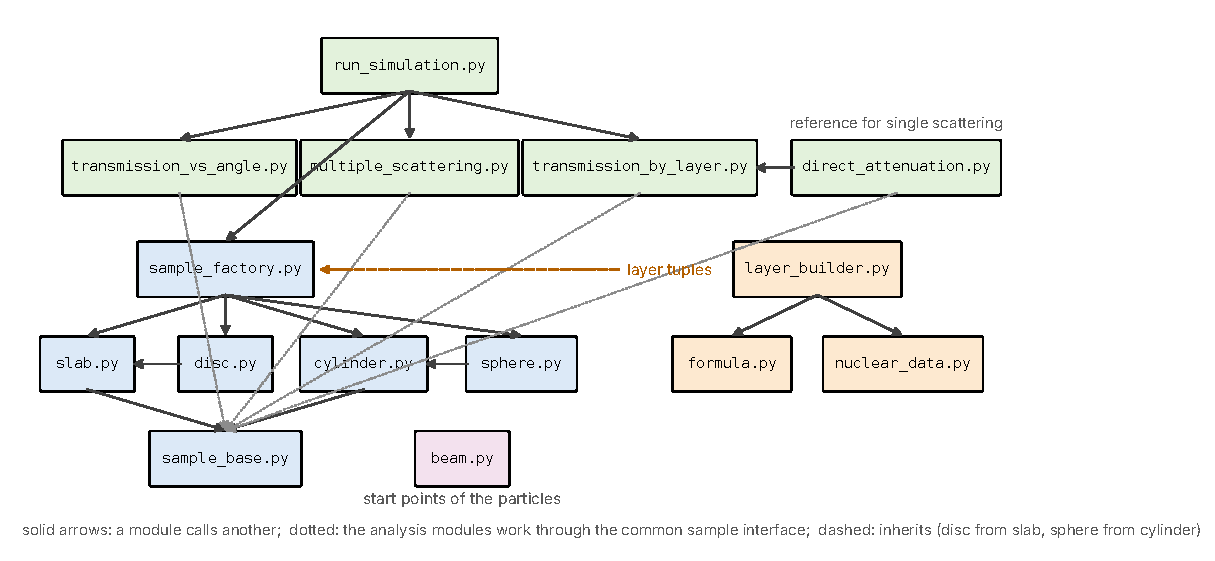
\includegraphics[width=0.95\textwidth]{fig_modules}
  \caption{The modules of the package and how they depend on each other. The
  analysis modules (green) work with any sample (blue) through the common interface
  defined in \texttt{sample\_base.py}; the modules in orange prepare the data of the layers.}
  \label{fig:modules}
\end{figure}

\begin{table}[ht]
  \centering\small
  \begin{tabular}{@{}p{4.6cm}p{10.2cm}@{}}
    \toprule
    \textbf{File} & \textbf{Content} \\ \midrule
    \code{beam.py}                 & Random start points of the particles in a rectangular beam, with optional profiles $H(x)$ and $V(y)$. \\
    \code{sample_base.py}          & The \code{Layer} record (with its filling), the abstract class \code{LayeredSample} (the common interface, vertical extent and filling of the layers) and \code{scattered_direction}. \\
    \code{slab.py}                 & Slab geometry: \code{SlabSample} and \code{create_slab_sample}. \\
    \code{disc.py}                 & Disc geometry (version 2.3): \code{DiscSample} (a \code{SlabSample} with a circular section) and \code{create_disc_sample}. \\
    \code{sphere.py}               & Sphere geometry (version 2.4): \code{SphericalSample} (a \code{CylindricalSample} with spherical surfaces) and \code{create_spherical_sample}. \\
    \code{cylinder.py}             & Cylindrical geometry: \code{CylindricalSample} and \code{create_cylindrical_sample}. \\
    \code{sample_factory.py}       & \code{make_sample}: builds a slab, a disc, a cylinder or a sphere from a name. \\
    \code{transmission_vs_angle.py}& Transmission of the scattered particles versus $2\theta$. \\
    \code{multiple_scattering.py}  & Particle-by-particle simulation: single and multiple scattering versus $2\theta$. \\
    \code{transmission_by_layer.py}& Transmission versus $2\theta$, one curve per layer of last scattering. \\
    \code{direct_attenuation.py}  & Direct method: single-scattering attenuation factors with exact weights, the same from the Monte Carlo, comparison. \\
    \code{formula.py}              & Reader of chemical formulas, with isotopes. \\
    \code{nuclear_data.py}         & Atomic masses and (optional) tabulated neutron cross sections. \\
    \code{layer_builder.py}        & Computes $\mu$ and the scatter fraction of a layer from formula, density and cross sections. \\
    \code{run_simulation.py}       & Main script: chooses the geometry and runs the whole chain. \\ \bottomrule
  \end{tabular}
  \caption{Files of the package.}
  \label{tab:files}
\end{table}

\section{A first look}

Everything below can be run from the folder that contains the modules. The quickest way to see
the package at work is the main script (Chapter~\ref{ch:main}), which builds an example sample,
computes the three kinds of results and saves the plots:
\begin{lstlisting}[style=shell]
python run_simulation.py --geometry slab
python run_simulation.py --geometry cylinder
python run_simulation.py --geometry cylinder --fullness 0.5
python run_simulation.py --geometry cylinder --bottom -6 --height 5
python run_simulation.py --geometry disc --plane-angle 45
python run_simulation.py --geometry sphere
\end{lstlisting}
From Python, the same chain is available as a function:
\begin{lstlisting}
from run_simulation import run_simulation
results = run_simulation("cylinder", n_particles=200000, show=False)
\end{lstlisting}
The rest of the manual explains each step separately.

\section{Notation used in this manual}

Names of files, functions and variables are written in \code{typewriter}. Mathematical symbols are listed
in Appendix~\ref{app:symbols}. Results shown as examples were obtained with the example samples of the
main script: they are illustrative, and the layer data (attenuation coefficients and scatter fractions)
are not those of a real experiment.
